\section{Results and Discussion}
\label{sec:results}
\begin{table}[!t]
	\centering
	\caption {Resource utilization of the proposed architecture for 16$\times$16 implementation when targeting Xilinx Ultrascale+ VU9P} 
	\begin{tabular}{l|l|l|l}
		\toprule
		Module Name        & Slice LUTs & Slice Regs & Memory Block \\
		\midrule
		Network Interface  & 322        & 251        & 0              \\
		Processing Element & 7          & 7          & 0              \\
		Switch             & 299        & 351        & 0              \\
		\midrule
		Total per node     & 628        & 609        & 0              \\
		\midrule
		{\bf Total Network}      & {\bf 159710}     &  {\bf 156290}    & {\bf 0}              \\
		\bottomrule
	\end{tabular}
	\label{tab:util}
\end{table}

\begin{figure}[!t]
\centering     %%% not \center
\subfigure[{\tiny Software: ER $\beta$= 0.1 $\gamma$= 0.3}]{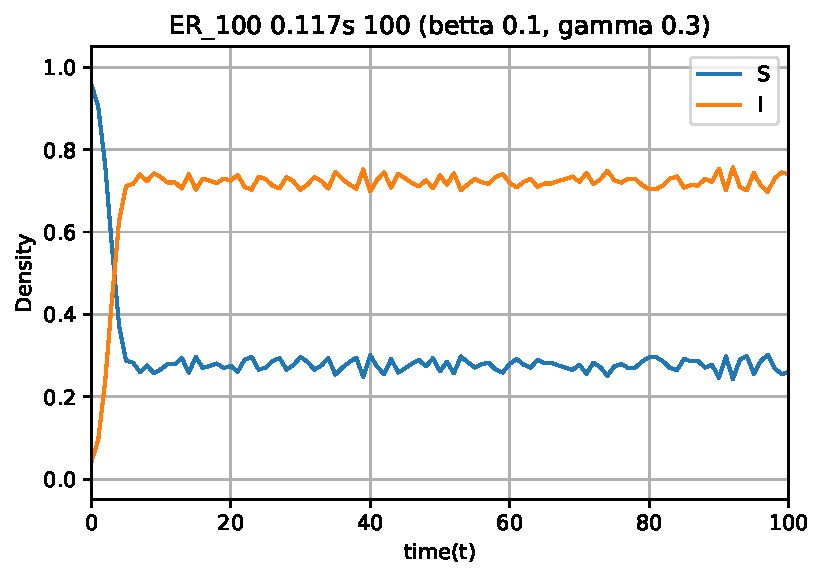
\includegraphics[width=0.32\columnwidth]{plots/10x10/ER100betta01gamma03.pdf}}
\subfigure[{\tiny Software: ER $\beta$= 0.5 $\gamma$= 0.2}]{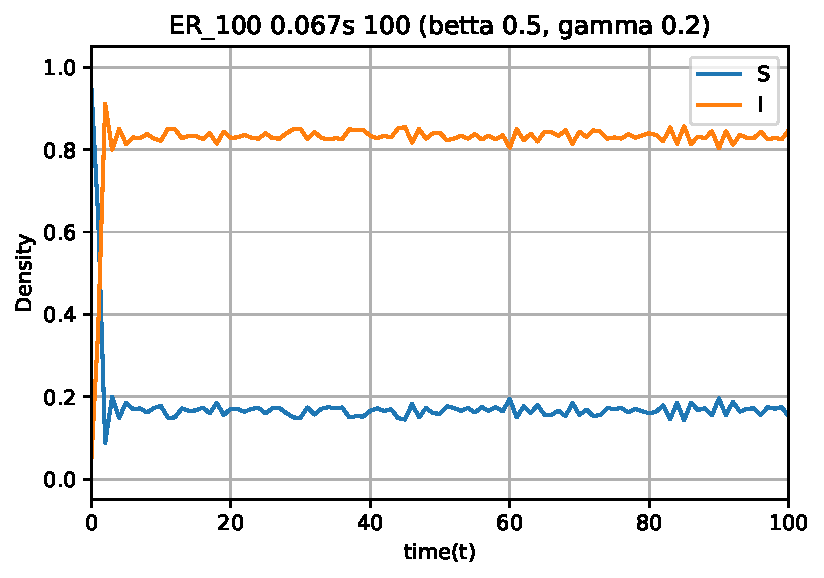
\includegraphics[width=0.32\columnwidth]{plots/10x10/ER100betta05gamma02.pdf}}
\subfigure[{\tiny Software: ER $\beta$= 0.7 $\gamma$= 0.9}]{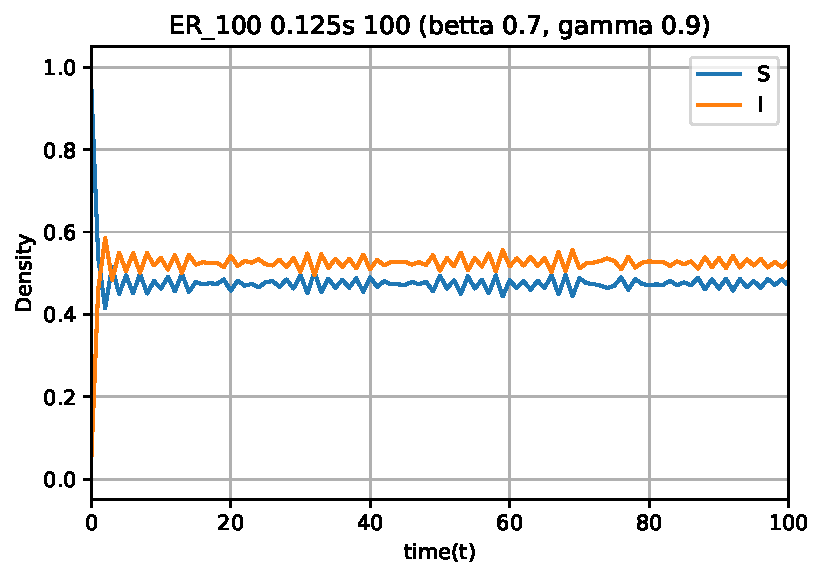
\includegraphics[width=0.32\columnwidth]{plots/10x10/ER100betta07gamma09.pdf}}

\subfigure[{\tiny Hardware: ER $\beta$= 0.1 $\gamma$= 0.3}]{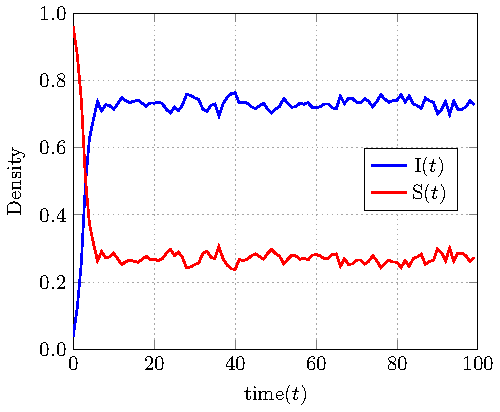
\includegraphics[width=0.32\columnwidth]{plots/10x10/ER100output3010.pdf}}
\subfigure[{\tiny Hardware: ER $\beta$= 0.5 $\gamma$= 0.2}]{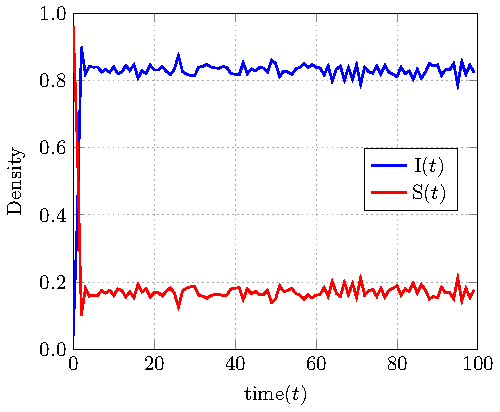
\includegraphics[width=0.32\columnwidth]{plots/10x10/ER100output2050.pdf}}
\subfigure[{\tiny Hardware: ER $\beta$= 0.7 $\gamma$= 0.9}]{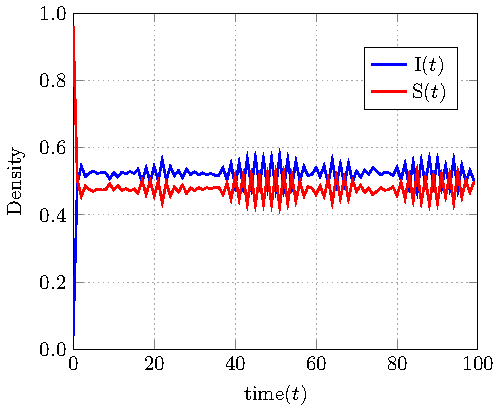
\includegraphics[width=0.32\columnwidth]{plots/10x10/ER100output9070.pdf}}

\subfigure[{\tiny Software: BA $\beta$= 0.1 $\gamma$= 0.3}]{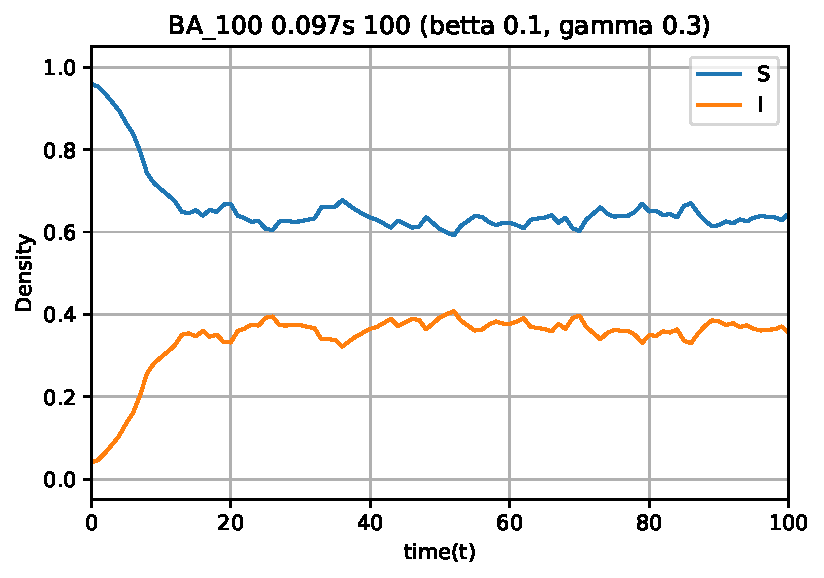
\includegraphics[width=0.32\columnwidth]{plots/10x10/BA100betta01gamma03.pdf}}
\subfigure[{\tiny Software: BA $\beta$= 0.5 $\gamma$= 0.2}]{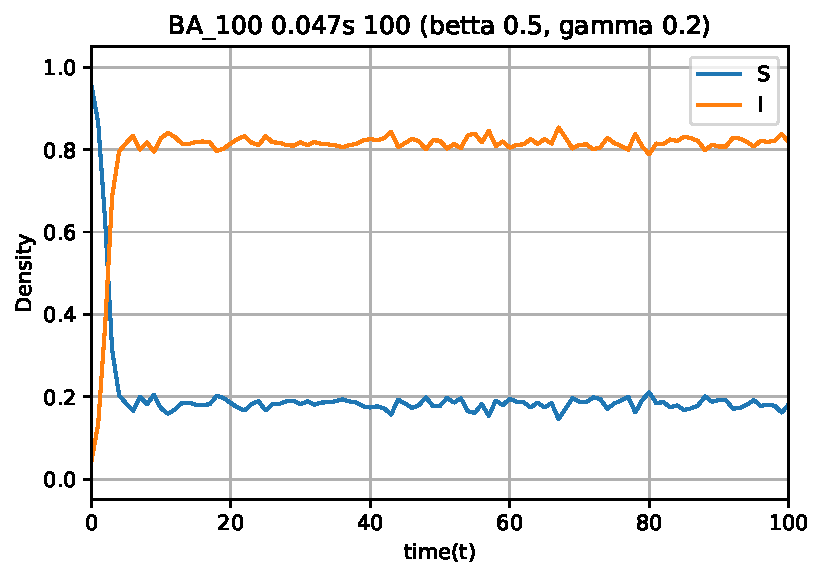
\includegraphics[width=0.32\columnwidth]{plots/10x10/BA100betta05gamma02.pdf}}
\subfigure[{\tiny Software: BA $\beta$= 0.7 $\gamma$= 0.9}]{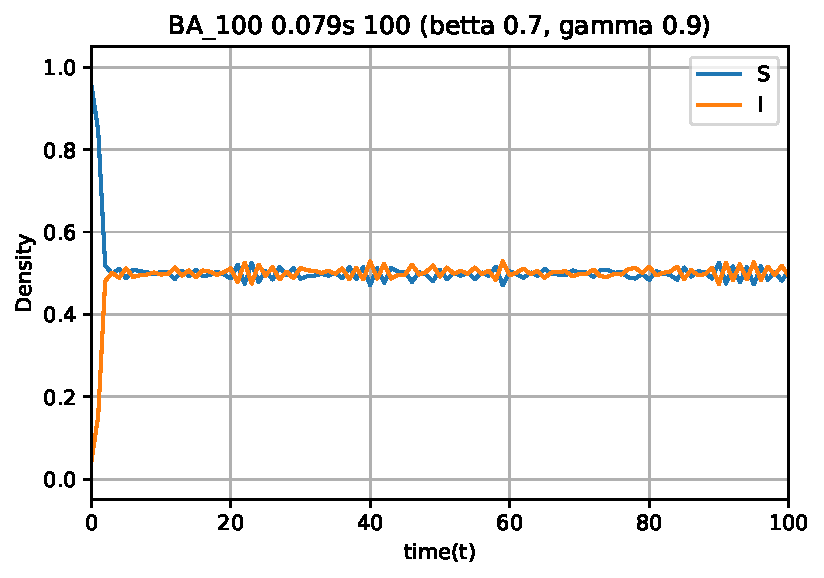
\includegraphics[width=0.32\columnwidth]{plots/10x10/BA100betta07gamma09.pdf}}

\subfigure[{\tiny Hardware: BA $\beta$= 0.1 $\gamma$= 0.3}]{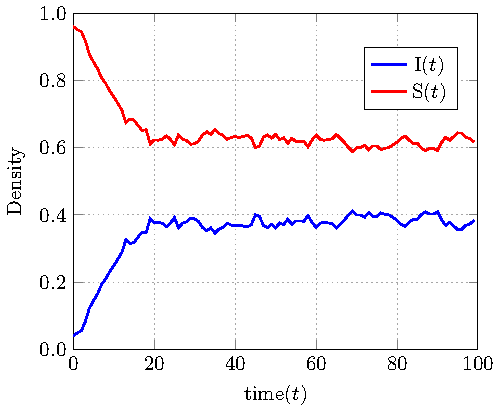
\includegraphics[width=0.32\columnwidth]{plots/10x10/BA100output3010.pdf}}
\centering     %%% not \center
\subfigure[{\tiny Hardware: BA $\beta$= 0.5 $\gamma$= 0.2}]{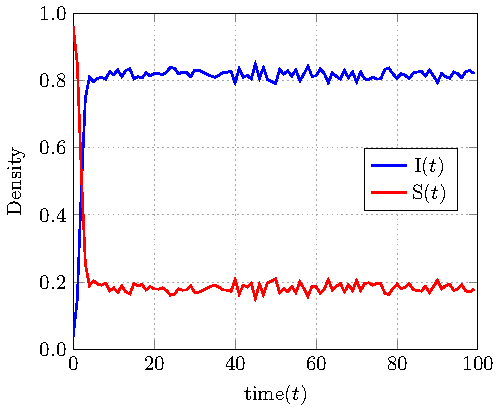
\includegraphics[width=0.32\columnwidth]{plots/10x10/BA100output2050.pdf}}
\subfigure[{\tiny Hardware: BA $\beta$= 0.7 $\gamma$= 0.9}]{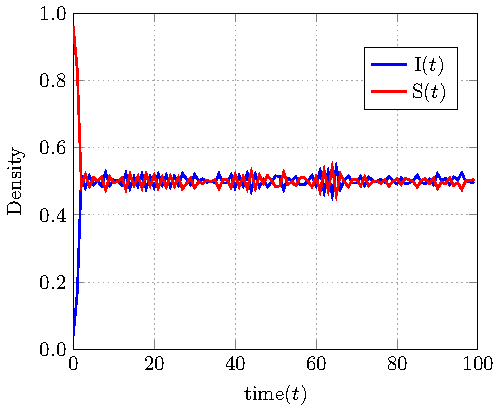
\includegraphics[width=0.32\columnwidth]{plots/10x10/BA100output9070.pdf}}
\end{figure}

\begin{figure}[!t]
\subfigure[{\tiny Software: WS $\beta$= 0.1 $\gamma$= 0.3}]{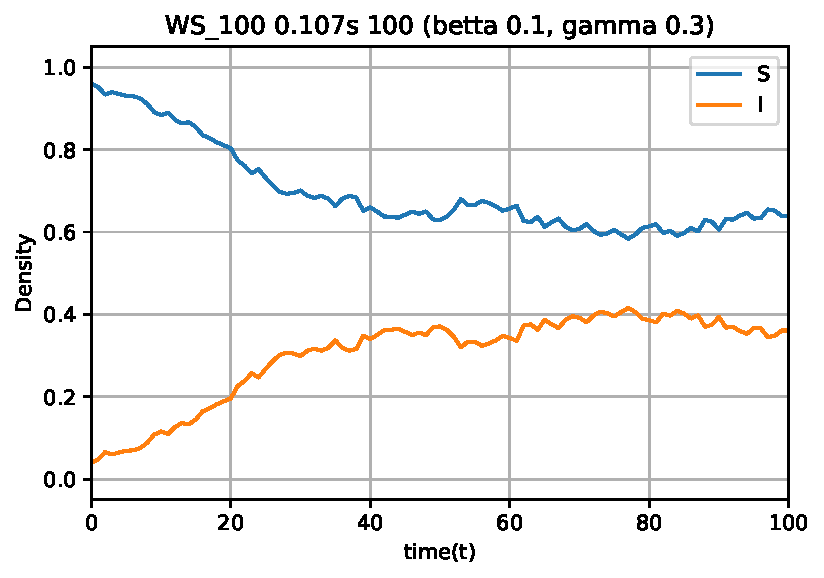
\includegraphics[width=0.32\columnwidth]{plots/10x10/WS100betta01gamma03.pdf}}
\subfigure[{\tiny Software: WS $\beta$= 0.5 $\gamma$= 0.2}]{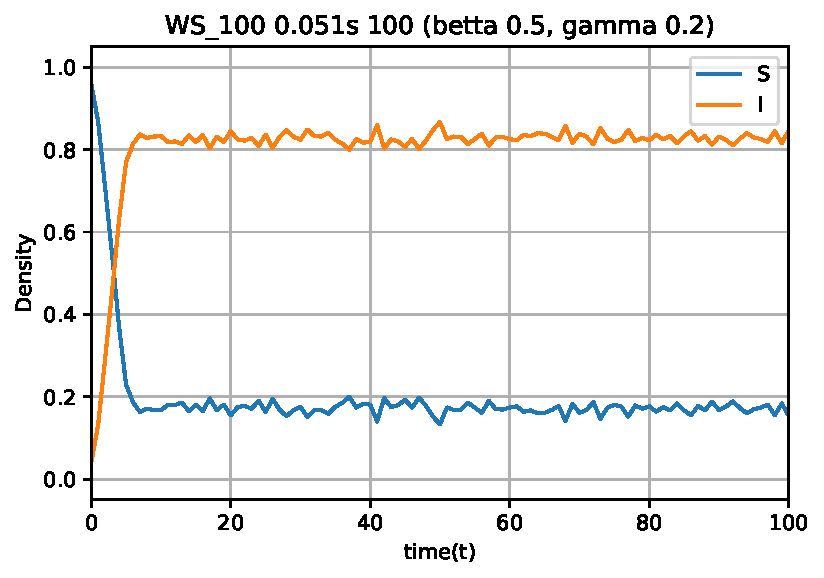
\includegraphics[width=0.32\columnwidth]{plots/10x10/WS100betta05gamma02.pdf}}
\subfigure[{\tiny Software: WS $\beta$= 0.7 $\gamma$= 0.9}]{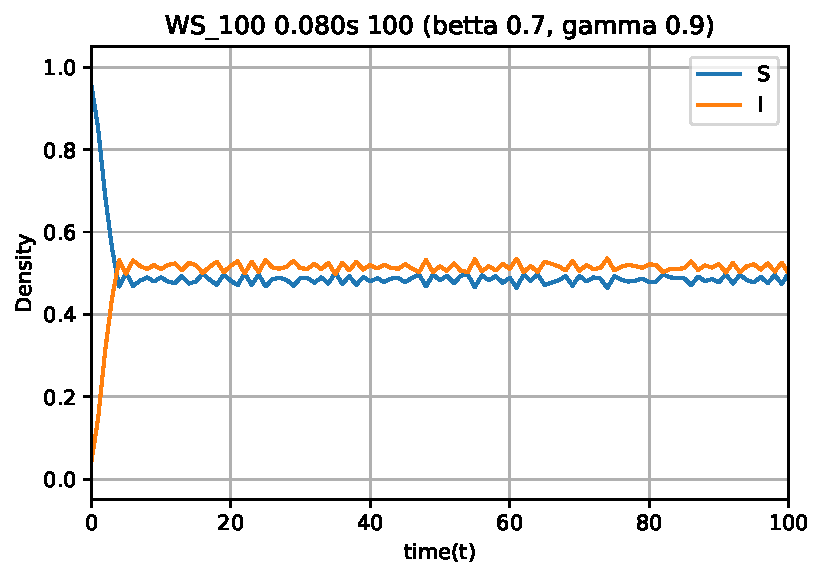
\includegraphics[width=0.32\columnwidth]{plots/10x10/WS100betta07gamma09.pdf}}

\subfigure[{\tiny Hardware: WS $\beta$= 0.1 $\gamma$= 0.3}]{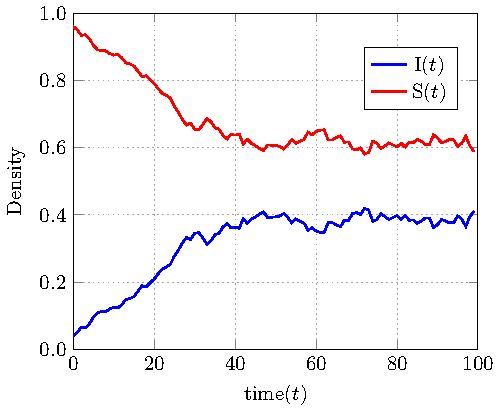
\includegraphics[width=0.32\columnwidth]{plots/10x10/WS100output3010.pdf}}
\subfigure[{\tiny Hardware: WS $\beta$= 0.5 $\gamma$= 0.2}]{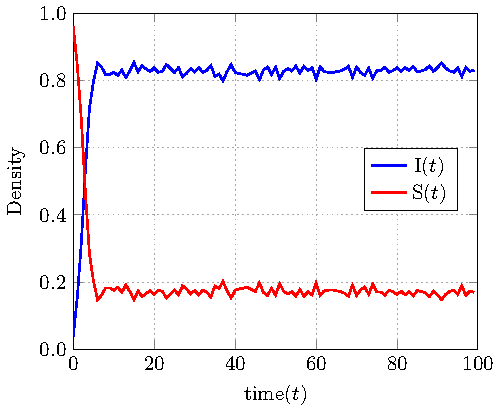
\includegraphics[width=0.32\columnwidth]{plots/10x10/WS100output2050.pdf}}
\subfigure[{\tiny Hardware: WS $\beta$= 0.7 $\gamma$= 0.9}]{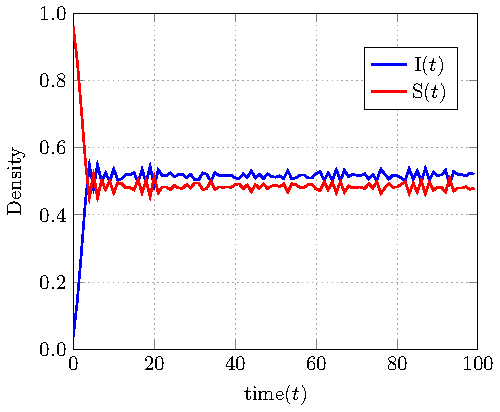
\includegraphics[width=0.32\columnwidth]{plots/10x10/WS100output9070.pdf}}
\caption{Comparison of software simulation and hardware simulation outputs for different $\beta$ and $\gamma$ values in a $10 \times 10$ network.}
\label{fig:results}

\end{figure}

The proposed platform is designed with Verilog HDL and implemented on a Xilinx Ultrascale+~VU9P device targeting Amazon AWS cloud-based FPGA instances.
Module-wise utilization for important building blocks and the overall utilization for a $16 \!\times 16$ network ($256$ nodes) is given in Table~\ref{tab:util}.
The implementation consumes about $8\%$ LUTs and $3\%$ of flip-flops on the target device.
At this rate, a network of $3000$ nodes can be supported on this device after reserving enough resources for the communication infrastructure (AWS shell infrastructure). 
FPGA architecture-dependent resources such as BRAM/URAM tiles of DSP slices are not utilized making the design highly portable to other platforms such as the Microsoft Azure or on-premises implementations.
Due to the heavily pipe-lined implementation, the platform can support to up to $260$MHz clock frequency, but is restricted to $250$MHz due to the PCIe-based host system interface.   

We first verified the validity and the functional correctness of the proposed platform by comparing its output with corresponding software-based implementation of the discrete SIS model.
Tests were conducted for three different network sizes ($10 \times 10$, $16 \times 16$, and $32 \times 32$) for three $\beta$ and $\gamma$ values and three different topologies, thus giving a total of $27$ test cases.
Results from each test case were averaged over $10$ runs to avoid outliers.
Software and hardware test outputs corresponding to a $10 \times 10$ implementation (network with $100$ nodes) with different rate and topology configurations shown in \figurename{~\ref{fig:results}}. It reveals that the steady state behavior and the number of discrete steps required to reach the steady state are similar in both cases which validates the functional correctness of the platform.

Table~\ref{tab:latency} compares the total run-time of software and the corresponding NoC-based implementations for modeling $100$ discrete time steps for different network models and sizes.
The software runs on an \emph{AWS EC2 a1.xlarge} cloud compute instance with $4$ vCPUs and $8$ GB RAM.
The NoC runs on an \emph{AWS f1.2xlarge FPGA} at $200$ MHz clock frequency.
The FPGA run-time includes the time required for configuring the RT each time before starting the simulation.
In a practical scenario, this could be avoided as long as the network topology remains intact.
The run-time for $10\times10$ and $16\times16$ are very similar for NoC implementation since the $10\times10$ implementation is physically a $16\times16$ implementation mapped using appropriate adjacency matrix.
This also shows the flexibility of the NoC architecture where a sub-network with any topology can be mapped to a mesh architecture using appropriate adjacency matrix. 
It is evident from the data that hardware outperforms software by an order of $2$ to $3$.
Considering the hourly rate of $0.102$~USD for a1.xlarge instance and $0.76-1.65$~USD for (based on subscription type) for f1.2xlarge instance, hardware acceleration can provide considerable financial benefits to users. 
\begin{table}[!t]
	\centering
	\caption {Wall clock time required for simulating 100 discrete time steps in software and proposed implementation} 
	\begin{tabular}{l|l|l|l|l}
		\toprule
		\multirow{ 2}{*}{\bf Topology}        & \multirow{ 2}{*}{\bf Run time(ms)}           & \multicolumn{3}{c}{\bf Network Size} \\
		\cline{3-5}
		&                              & {\bf 100} & {\bf 256} & {\bf 1024}     \\
		\midrule
		\multirow{ 2}{*}{WS}  & Software   & 107       & 312    & 1297 \\
		                      & NoC        & 0.213     & 0.232  & 2.81 \\
		\midrule
		\multirow{ 2}{*}{BA}  & Software   & 97        & 242    &  1130 \\
		                      & NoC        & 0.215     & 0.248  &  2.78 \\
		\midrule
		\multirow{ 2}{*}{ER}  & Software   & 117       & 473    & 4408\\
		                      & NoC        & 0.217     & 0.262  & 3.67\\
		\bottomrule
	\end{tabular}
\label{tab:latency}
\end{table}

One of the main limitations of NoC-based implementation of network models is the size of the supported network size.
Even with modern FPGAs with multi-million equivalent gate capacity, networks with a few thousand nodes can be supported.
Modeling large networks such as social media will require implementation of networks with millions of nodes.
In a cloud environment, multiple FPGAs can be combined to simulate larger networks.
Communication between the FPGAs will be managed by the cloud communication infrastructure.
Two other approaches can be used for overcoming this limitation for resource constrained FPGAs.  
Using partial reconfiguration, FPGA resources can be time multiplexed and portions of the network can be simulated during different time instances and results can be combined to determine the total network performance.
Another method is through structural reconfiguration, where portions of the network is configured through modifying network parameters such as the PE address.
Intermediate result for each configuration is stored in external memory and broadcasted to the network after reconfiguration.
 